\section{Query optimization}

\begin{figure}[h!]
		\centering
		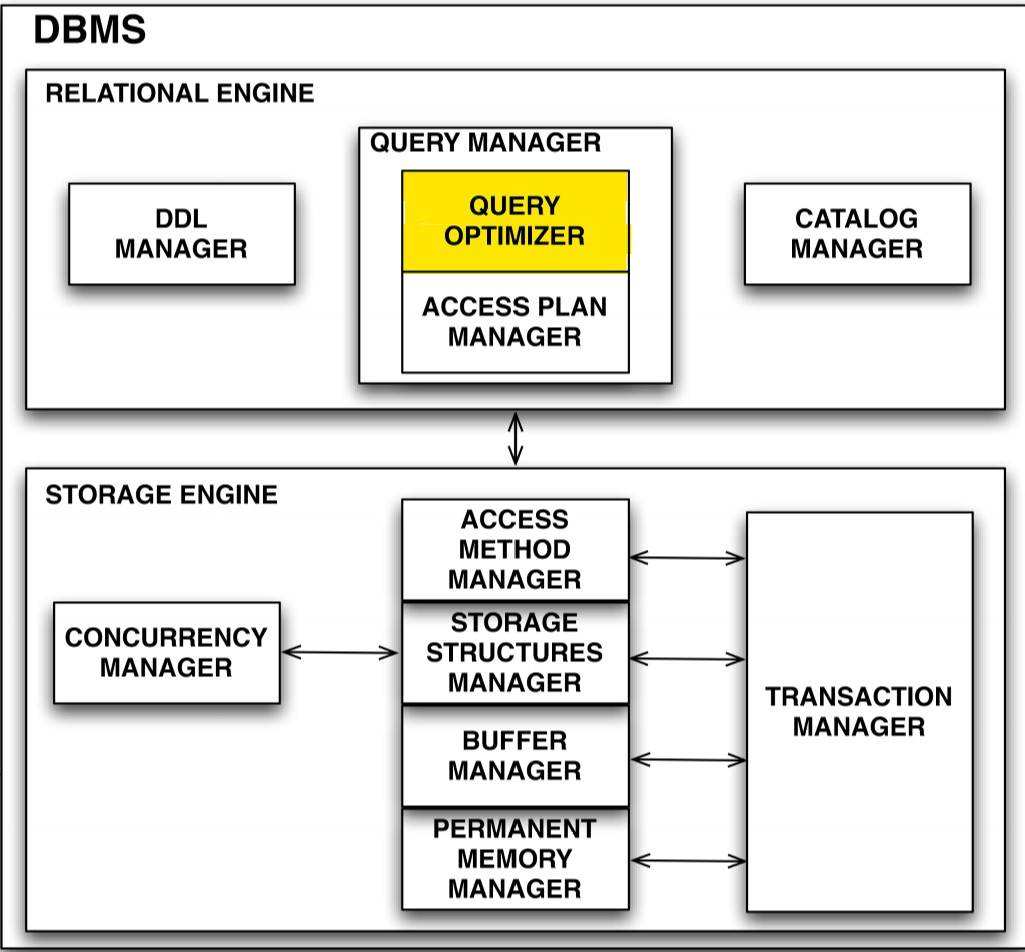
\includegraphics[scale = 0.7]{img/queop1.jpg}
		\label{relop13}
\end{figure}

In this chapter the focus is on query processing and on how to find the best plan to execute a query. In particular, we study the optimizer organization, a fundamental component of the \textbf{Query Manager}, which selects the optimal physical plan to execute queries using the operators and data structures of the Storage Engine. We will also show how functional dependencies, well known for relational schema design, are also important for query optimization.

\subsection{Introduction}
The \textbf{goal} of the optimizer is to find an efficient plan to execute a query. This problem is complex because:

\begin{itemize}
    \item a query can be written in several equivalent ways;
    \item a relational algebra operator can be implemented with different physical operators.
\end{itemize}

, so the optimizer will use some heuristic methods to find a good solution quickly.

The optimization can be:
\begin{itemize}
    \item \textbf{dynamic}, i.e. the physical plan is generated at run time when the query is executed, taking into account some informations about the DB and the available data structures;
    \item \textbf{static}, i.e. the physical plan in generated at the program compilation time
\end{itemize}

\subsubsection{Query processing phases}
\begin{enumerate}
    \item \textbf{query analysis}: the correctness of the SQL query is checked and it is transformed into relational algebra, i.e. the \textit{initial logical query plan}
    \item \textbf{query transformation}: the initial logical plan is transformed into an equivalent one that provides a better query performance
    \item \textbf{physical plan generation}: alternative algorithms for the query execution are considered and the \textit{physical query plan} with the lowest cost is chosen. This step makes query processing hard, because there's a large number of alternative solutions to consider in order to choose the best one
    \item \textbf{query evaluation}: the physical plan is executed
\end{enumerate}

\subsection{Query analysis phase}
\begin{enumerate}
    \item lexical and syntax query analysis
    \item semantic query analysis, in which the system check both the query semantic correctness and that the user has appropriate privileges
    \item simplification of the \textbf{WHERE} condition using:
    \begin{itemize}
        \item equivalence rules of boolean expressions;
        \item elimination of contradictory conditions;
        \item elimination of NOT conditions;
    \end{itemize}
    \item generation of the internal representation of the query as an \textbf{initial logical query plan}, represented as an expression tree of relational algebra operations. For example, the query: 

    \begin{figure}[h!]
		\centering
		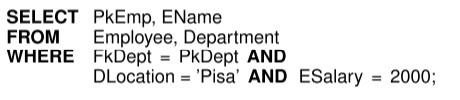
\includegraphics[scale = 1.3]{img/queop2.jpg}
		\label{relop13}
    \end{figure}

    is transformed into the following logical plan:

    \begin{figure}[h!]
		\centering
		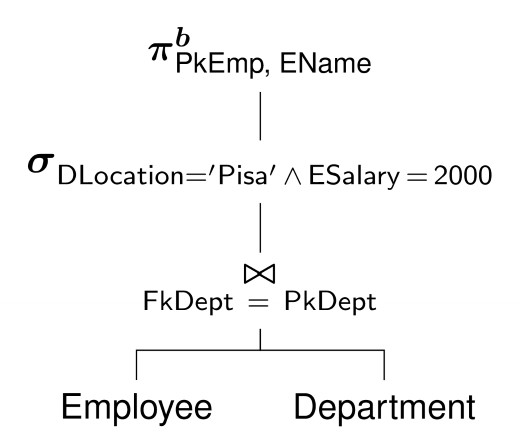
\includegraphics[scale = 0.9]{img/queop3.jpg}
		\label{queop3}
        \caption{Initial logical query plan}
    \end{figure}
    
\end{enumerate}

\subsection{Query transformation phase}
In this phase, the \textit{initial logical query plan} is transformed into an equivalent one using a set of equivalence rules, for example the \textit{cascading of selections} or the \textit{commutativity of selection and projection}. In general, the following rules are followed:

\begin{itemize}
    \item selections are pushed below projections and they're grouped;
    \item selections and projections are pushed below joins;
    \item unnecessary projections are deleted;
    \item projections are grouped.
\end{itemize}

Picture \ref{queop4} shows an example of transformation of the initial logical query plan of Picture \ref{queop3}.

\begin{figure}[h!]
		\centering
		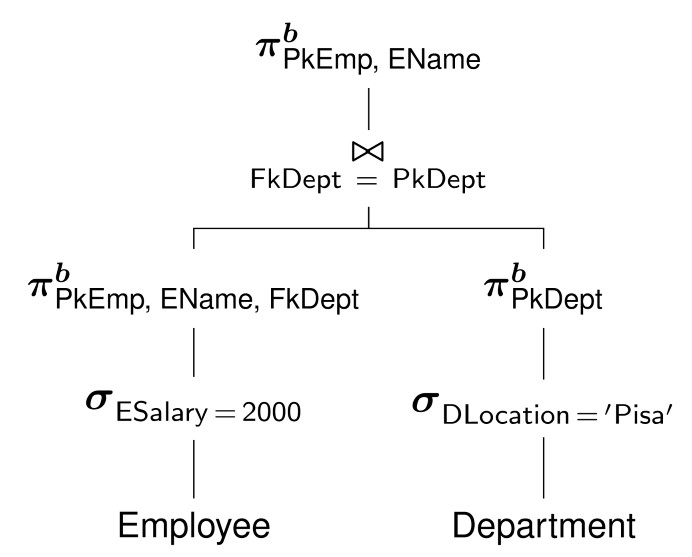
\includegraphics[scale = 0.9]{img/queop4.jpg}
		\label{queop4}
        \caption{Transformation of the initial logical query plan}
\end{figure}

\subsubsection{DISTINCT elimination}
The DISTINCT operation requires SORT, which is costly, so we use the functional dependencies theory to discover if an interesting functional dependency can be inferred into the result of a query. In general, let $A$ be the set of attributes of the result and $K$ be the union of the attributes of the key of every table used in the query, then if $A -> K$, then the operator $\delta$ for duplicate elimination is unnecessary.

\subsubsection{GROUP BY elimination}
As DISTINCT, also GROUP BY requires the SORT operation. In this case, the elimination can happen:
\begin{itemize}
    \item if there's only a single group;
    \item each group is composed of a single tuple
\end{itemize}

\subsubsection{WHERE-subquery elimination}
In general, to execute such queries, the optimizer generate a physical plan for the subquery, which then will be executed for each record processed by the outer query. Therefore, the presence of a \textbf{subquery} makes the \textbf{physical plan more expensive}, and for this reason techniques have been studied to transform a query into an equivalent one without the subquery, which the optimizer processes more efficiently. In particular, all the subqueries can be rewritten using EXISTS and NOT EXISTS, and in certain cases they can be eliminated with the introduction of JOIN.

\begin{figure}[h!]
		\centering
		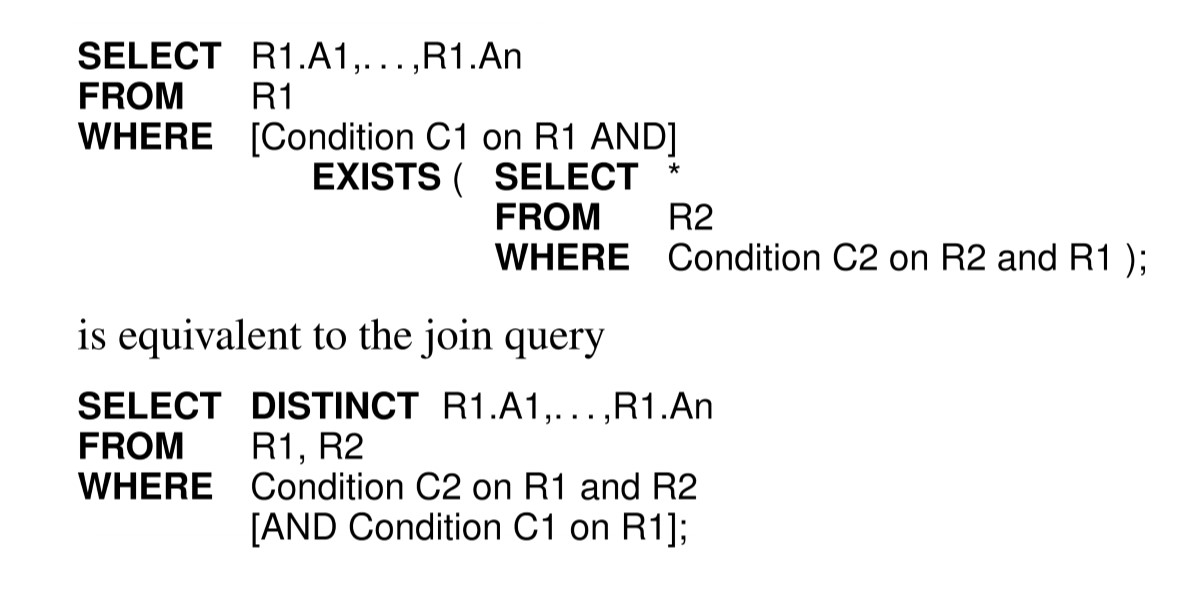
\includegraphics[scale = 0.9]{img/queop5.jpg}
		\label{queop4}
\end{figure}

\textbf{NOTE}: by using the join we create all the possible pairs, so we must check for DISTINCT!

Complex queries are much easier to write and understand if \textbf{views} are used, either by creating them with \textbf{CREATE VIEW} or by using \textbf{WITH} (the second one creates temporary views available only to the query in which the clause occurs).In general, when a query uses a view, the optimizer generates a physical sub-plan for the SELECT that defines the view, and optimizes the query considering the scan as the only access method available for the result of the view.


\subsection{Physical plan generation phase}
The goal of this phase is to find a plan to execute a query, among the possible ones, which has the \textbf{minimum cost} on the basis of the available information on storage structures and statistics. The main steps of this phase are:

\begin{itemize}
    \item generation of alternative physical query plans;
    \item choice of the physical query plan with the lowest estimated cost.
\end{itemize}

To estimate the cost of a physical query plan it is necessary to estimate, for each node in the physical tree:

\begin{itemize}
    \item the cost of the physical operator;
    \item the size of the result and if the result is sorted.
\end{itemize}
 
Let's see an example of alternative physical plans for a query and their
cost. Let's consider a DB and the following query:

\begin{figure}[H]
		\centering
		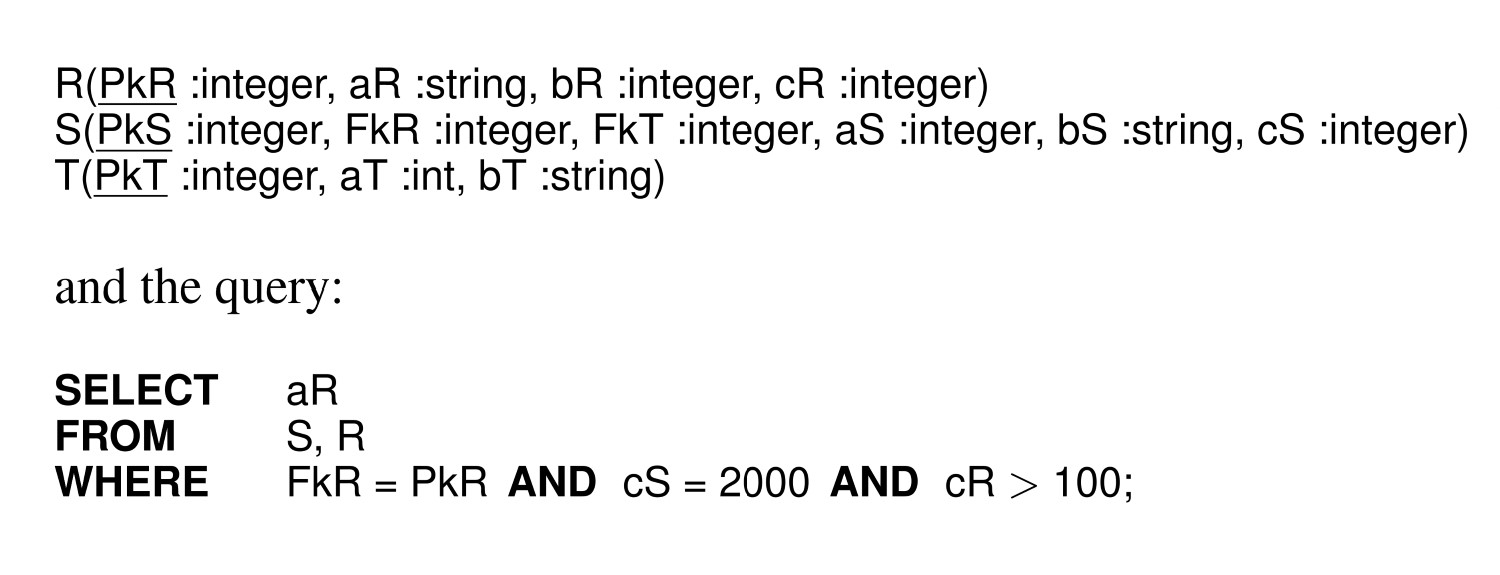
\includegraphics[scale = 0.7]{img/queop6.jpg}
		\label{queop4}
\end{figure}

, and let's consider two alternative physical query plans: the first one uses the join operator \textbf{PageNestedLoop}, while the second one uses the available \textbf{indexes}.

\begin{figure}[H]
		\centering
		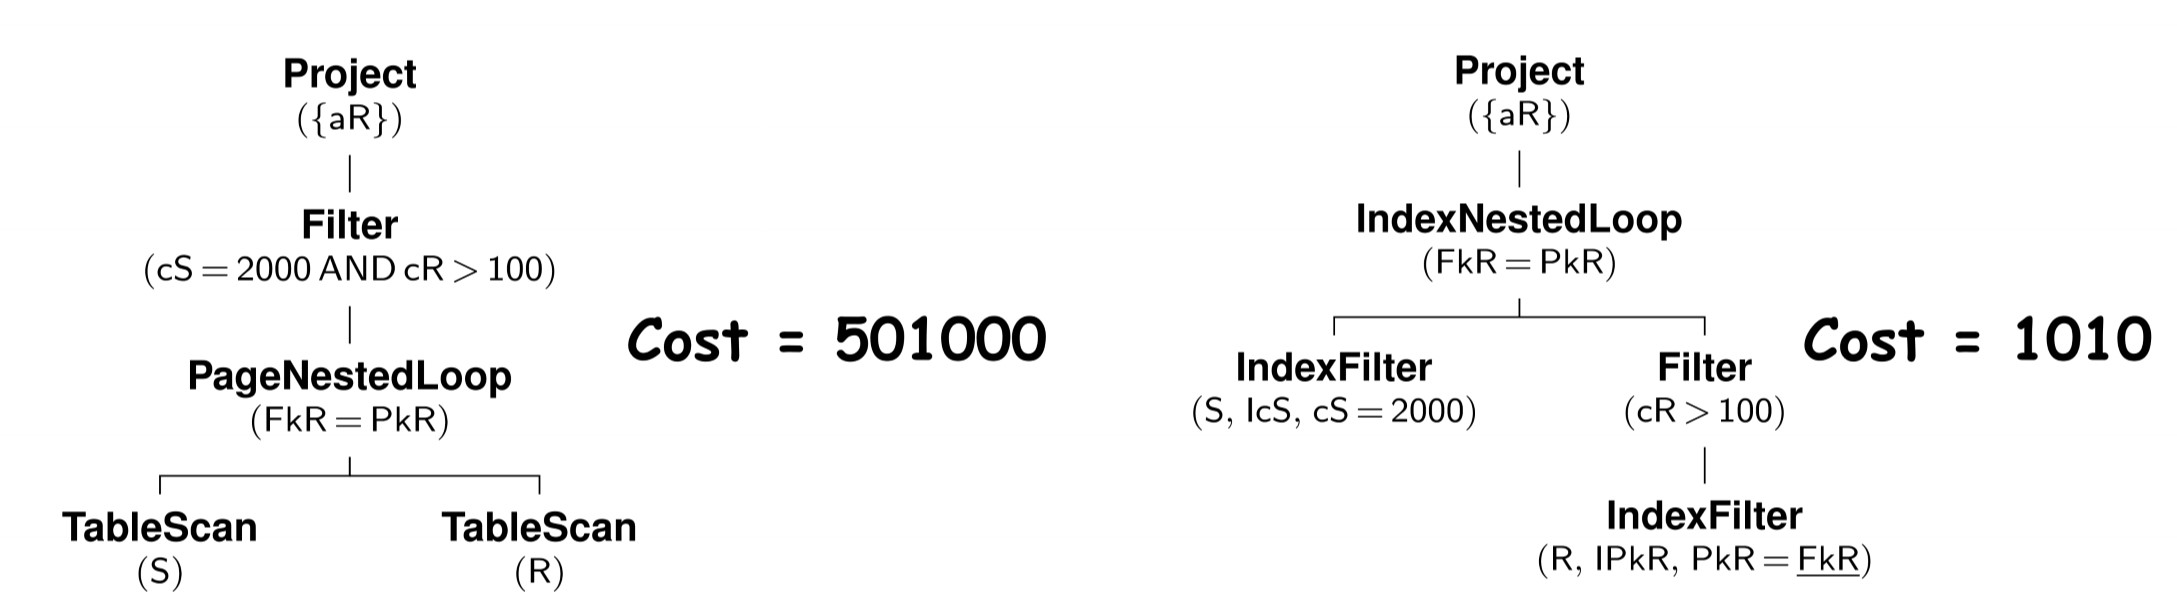
\includegraphics[scale = 0.7]{img/queop7.jpg}
		\label{queop4}
\end{figure}

Clearly, the second physical plan has better performances than the first one.

\subsubsection{Single relation queries}
If the query uses just one relation, the operations involved are the projection and selection.

If there are \textbf{no useful indexes}, the solution is to perform a scan + projection.

Otherwise, if there are useful index we can:

\begin{itemize}
    \item \textbf{use of single-index}: the one of minimal cost is used, and it tests if the record satisfy the conditions and projection is applied. Note that the records of the result are sorted on the index attribute;
    
    \item \textbf{use of multiple-indexes}: the operation is completed by testing whether the retrieved records satisfy the remaining conditions and the projection is applied;

    \item \textbf{use of index-only}: if all the attributes of the condition of the SELECT are included in the prefix of the key of an index, the query can be evaluated using only the index with the query plan of minimum cost.
    
\end{itemize}

\subsubsection{Multiple relation queries}
Queries with two or more relations in the FROM clause require joins (or crossproducts), and finding a good physical query plan for these queries is very important to improve their performances. 

In the following, for simplicity, we will consider an optimization algorithm based on the idea of generating and searching a \textbf{state space} of possible solutions to find the one with minimal cost. The state space is constructed step-by-step starting with an initial state and repeatedly applying a set of operators to expand a state $s$ into other ones, called the \textit{successors} of $s$. Each state $s$ corresponds to a relational algebra subexpression of a given query $Q$ to optimize, and the successors of s are larger subexpressions of Q. The cost of a state $s$ is that of the best physical plan to execute the expression associated to $s$. 

The state space is represented as a tree of nodes, where the root is the empty subexpression, the first level nodes are the query relations or selections and projections on each of them; the following levels are alternative joins of the algebraic expressions of the previous level. The node of the “optimum” state is the expression the contains all the query joins, which is then extended with other operators (e.g. project, sort or group by) to become the final state of the query expression, with the associated minimal cost physical query plan. 

As queries become more complex, the full search algorithm cannot find the overall best physical query plan in a reasonable amount of time because of the \textbf{exponential nature of the problem}. Therefore, several \textbf{heuristics} have been proposed in the DBMS literature that allow the query optimizer to avoid bad query plans and find query plans that, while not necessarily optimal, are usually “good enough”. Some examples are \textit{limitation of the number of successors}, \textit{greedy search} and so on..

\subsubsection{Other queries}

\begin{itemize}

    \item \textbf{DISTINCT queries}: assuming that the operation is performed by sorting, the physical plan for a SELECT ORDER BY is generated, and then extended with the physical operator \textbf{Distinct(O)};
    
    \item \textbf{GROUP BY queries}: the optimizer produces a physical plan for the SELECT only, without considering the GROUP BY clause, which produces the result sorted on the grouping attributes. The physical plan is then extended with a physical operator for the \textbf{GroupBy} and the operator \textbf{Project} over the SELECT attributes. If the SELECT has also a HAVING clause, the physical plan is extended with a selection operator, and the operator \textbf{GroupBy} computes all the aggregate functions used in the HAVING and SELECT clauses;

    \paragraph{Pre-grouping transformation}
    The standard way to evaluate join queries with grouping and aggregations is to perform the join first, but sometimes it is convenient to anticipate grouping operations. However, complex conditions are needed to perform this optimization, which also depends on the type of aggregate functions.

    \item \textbf{Queries with set operations}: we only consider the UNION operator. The optimizer is used to generate the physical plans for the two SELECT of the UNION, with duplicate elimination operators, which then become the operands of the \textbf{Union} operator.

    
\end{itemize}